\section{Materiales y métodos}
Se estudió la propagación de un pulso sinusoidal en una red de circuitos RC en escalera de 16 nodos, donde cada malla cuenta con una resistencia de \SI{2700(135)}{\ohm} y un capacitor de \SI{220(22)}{\nano\farad}, con el objetivo de obtener la impedancia caracteristica del arreglo RC \((Z)\) y determinar la constante temporal \(\tau=RC\). A su vez, se estudió la respuesta de un cable coaxial \(RG-58\) de \SI{100}{m} frente a un pulso de ondas cuadradas variando la impedancia de carga del sistema \(Z_L\) en tres situaciones distintas tal que \(Z_L = \infty\), dejando el circuito abierto,  \(Z_L = 0\) puenteando el circuito, y \(Z_L = Z_C\) siendo \(Z_C = 50(3)\) \si{\Omega} la impedancia caracteristica del circuito correspondiente a un coeficiente de reflexión \( \Gamma = \frac{Z_L - Z_C}{Z_L+Z_C} \), tal que \(\Gamma =1\), \(\Gamma=-1\) y \(\Gamma=0\), respectivamente \cite{RG58Cable}. Para cada una de las configuraciones, se observó el comportamiento de la onda reflejada respecto a la incidente según el coeficiente de reflexión y midiendo simultaneamente la diferencia de fase entre ambas \cite{Bobowski_2021}. Para obtener \(Z\) se midió la señal de la resistencia en el primer nodo y la fuente paulatinamente (Ver \autoref{fig:configNodoCte}).

La obtención de \(\tau\) se realizó con dos métodos, por un lado se mantuvo la frecuencia de la fuente constante a $50(1)$ \si{\hertz} y se midió la caída de tensión en cada nodo, por otro lado se varió la frecuencia de la fuente en un rango de \([0,500]\) \si{\hertz} midiendo la caída de tensión en el nodo 6 únicamente (Ver \autoref{fig:configFCte}). En el margen de bajas frecuencias y sin inductores la ecuación \eqref{eq:difV} se reduce a
\begin{equation}
    V(z,t) = V_0 e^{-\sqrt{\frac{\omega \tau}{2}}z} e^{i(\omega t - \sqrt{\frac{\omega \tau}{2}}z)}
    \label{eq:voltajePulso}
\end{equation}
Siendo \(V_0\) la amplitud del pulso, $\tau$ la constante de tiempo a determinar, \(z\) el nodo donde se mide y \(\omega\) la frecuencia angular de la fuente.  

Para ambas mediciones de \(Z\) y \(\tau\) se registró el desfasaje entre las señales con el objetivo de realizar un gráfico de Bode. Se utilizó como fuente una señal sinusoidal de amplitud constante mediante un generador de funciones $Sinometer$ modelo VC2002 \cite{VC2002}. Tanto la señal de entrada (\(V_0\)) como la de salida (\(V_S\)) se registraron a través de un osciloscopio $Tektronix$ modelo TDS 220 \cite{TDS200} (ver \autoref{fig:ambosCircuitos}).


\begin{figure}[h!]
    \centering
    \begin{subfigure}[b]{0.45\linewidth}
        \centering
        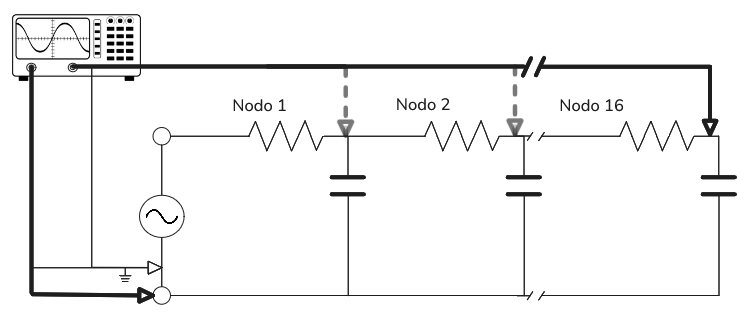
\includegraphics[width=\linewidth]{gráficos/ConfiguracionF.png}
        \caption{Configuración utilizada para obtener la constante de tiempo, donde para una frecuencia constante se midió cada nodo y para frecuencia variable se fijó el nodo 6.}
        \label{fig:configFCte}
    \end{subfigure}
    \hfill
    \begin{subfigure}[b]{0.40\linewidth}
        \centering
        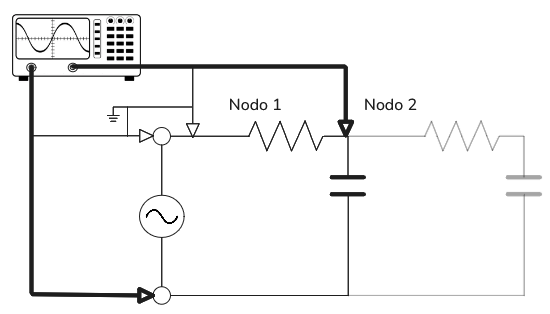
\includegraphics[width=\linewidth]{gráficos/Impedancia.png}
        \caption{Configuración utilizada para obtener la impedancia del circuito, donde se midió la diferencia de potencial entre la fuente y la resistencia del primer nodo.}
        \label{fig:configNodoCte}
    \end{subfigure}
    \caption{Esquemas del circuito utilizado para obtener la impedancia y la constante de tiempo del circuito.}
    \label{fig:ambosCircuitos}
\end{figure}
